\documentclass[UTF8,zihao=-4]{ctexart}
\usepackage[a4paper,margin=1.9cm]{geometry}
\usepackage{hyperref}
\usepackage{array}
\usepackage{longtable}
\usepackage{verbatim}
\usepackage{xcolor}
\usepackage{graphicx}
\usepackage{tikz}
\usetikzlibrary{arrows.meta,positioning,fit,calc,shapes.geometric}
\hypersetup{hidelinks}
\setlength{\parindent}{0pt}
\setlength{\parskip}{0.45em}
\emergencystretch=4em
\sloppy
\tikzset{
  umlbox/.style={draw, rounded corners=2pt, align=center, minimum height=7mm, inner sep=3pt, font=\small},
  umlsmallbox/.style={draw, rounded corners=2pt, align=center, minimum height=6mm, inner sep=2pt, font=\scriptsize},
  umllifeline/.style={draw, align=center, minimum width=20mm, minimum height=7mm, inner sep=2pt, font=\scriptsize},
  umlmsg/.style={-{Latex[length=2mm]}, line width=0.45pt},
  umlreturn/.style={-{Latex[length=2mm]}, dashed, line width=0.45pt},
  umlrealize/.style={-{Triangle[open,length=3mm,width=3mm]}, dashed, line width=0.45pt},
  umlinherit/.style={-{Triangle[open,length=3mm,width=3mm]}, line width=0.45pt},
  packagebox/.style={draw, rounded corners=2pt, align=center, inner sep=5pt, font=\small},
  usecase/.style={draw, ellipse, align=center, inner sep=2pt, font=\scriptsize, minimum height=8mm, text width=20mm},
  statebox/.style={draw, rounded corners=2pt, align=center, minimum height=7mm, inner sep=3pt, font=\scriptsize}
}
\newcommand{\umlactor}[1]{%
\begin{tabular}{c}

\begin{tikzpicture}[scale=0.38,baseline=-0.6ex]
\draw (0,0) circle (0.25);
\draw (0,-0.25) -- (0,-0.95);
\draw (-0.45,-0.55) -- (0.45,-0.55);
\draw (0,-0.95) -- (-0.4,-1.45);
\draw (0,-0.95) -- (0.4,-1.45);
\end{tikzpicture}\\[-0.2em]
#1
\end{tabular}}
\title{软工二最简综合卷与补充模拟卷}
\author{}
\date{}
\begin{document}
\maketitle
\setcounter{tocdepth}{1}
\tableofcontents
\newpage

\section{软件工程与计算 II 最简综合卷与补充模拟卷}


\subsection{使用说明}


本文件基于以下已读取材料整理：


\begin{itemize}
\item \texttt{Exam/答案整理/期末试题答案汇总.md}
\item \texttt{软工二期末突击/00-零基础期末总复习资料.md}
\item \texttt{软工二课程整理/课程框架与重点名词.md}
\item \texttt{Review/名词解释.pdf}
\item \texttt{Review/补充简答题.pdf}
\item \texttt{Review/复习提纲.pdf}
\item \texttt{Review/复习知识点.pdf}
\item \texttt{Review/summary-重点.pdf}
\item \texttt{软工二期末突击/模拟卷/模拟卷01-校园卡自助系统题目与详解.md}
\item \texttt{软工二期末突击/模拟卷/模拟卷02-进销存采购补货系统题目与详解.md}
\item \texttt{软工二期末突击/模拟卷/模拟卷03-教师排课系统题目与详解.md}
\item \texttt{软工二期末突击/模拟卷/模拟卷04-图书馆借阅预约系统题目与详解.md}
\item \texttt{软工二期末突击/模拟卷/模拟卷05-移动支付积分系统题目与详解.md}
\item \texttt{软工二期末突击/模拟卷/模拟卷06-在线选课系统题目与详解.md}
\item \texttt{软工二期末突击/模拟卷/模拟卷07-医院预约挂号系统题目与详解.md}
\item \texttt{软工二期末突击/模拟卷/模拟卷08-实验室设备预约报修系统题目与详解.md}
\end{itemize}


整理原则：


\begin{quote}
\footnotesize
\begin{verbatim}
1. 最简综合卷保留历年卷稳定十题结构，每类核心题型只出一次。
2. 补充模拟卷覆盖已有 8 套系统场景卷中训练较少的旧题和边角知识。
3. 答案按卷面可直接书写的格式给出，需要画图的题目直接给出图形，另配接口代码和测试表述。
\end{verbatim}
\end{quote}


\section{最简综合模拟卷}


\subsection{A 卷题目}


\subsubsection*{一、简答题（10 分）}


回答下列问题：


\begin{enumerate}
\item 软件工程的定义。
\item 软件配置管理中的变更控制过程。
\item 增量迭代模型和演化模型的区别。
\end{enumerate}


\subsubsection*{二、需求题（10 分）}


场景：学校建设 \texttt{校园服务预约与工单系统}，学生可以预约教室、自习室和实验设备，也可以提交维修工单。管理员负责审核资源、处理工单并查看统计报表。系统需要和统一认证、消息服务、资源管理系统交互。


完成：


\begin{enumerate}
\item 写出 2 个用例，说明参与者和主成功场景。
\item 写出一个业务需求、一个用户需求和一个系统级需求。
\item 判断“系统需要向资源管理系统提供 REST API 供调用”属于哪类需求，并说明原因。
\end{enumerate}


\subsubsection*{三、需求分析题（10 分）}


针对 \texttt{校园服务预约与工单系统}：


\begin{enumerate}
\item 识别问题域概念类。
\item 写出类之间的关联和多重性。
\item 画出一个系统顺序图，要求只把系统当成黑盒。
\end{enumerate}


\subsubsection*{四、体系结构设计题（10 分）}


系统采用 Web 分层架构：


\begin{enumerate}
\item 画出物理包图，要求体现客户端 \texttt{html/css/javascript/presentation}，服务器端 \texttt{controller}、\texttt{service}、\texttt{repository}、\texttt{domain}、\texttt{database}，并标注 \texttt{HTTP + REST API + JSON}。
\item 写出预约服务的 \texttt{Service} 接口、\texttt{Repository} 接口和 \texttt{Controller} 构造器注入代码片段。
\end{enumerate}


\subsubsection*{五、详细设计题（10 分）}


针对“提交预约申请”：


\begin{enumerate}
\item 画出 \texttt{Controller}、\texttt{Service}、\texttt{Repository}、外部消息服务之间的详细顺序图。
\item 简述集中式、委托式、分散式控制风格。
\item 判断该场景应采用的控制风格，并说明理由。
\end{enumerate}


\subsubsection*{六、模块化与信息隐藏题（10 分）}


系统中 \texttt{reservation}、\texttt{resource}、\texttt{workorder}、\texttt{notification}、\texttt{user} 包互相直接访问内部对象，且多个包直接读取同一个可变全局配置对象。


完成：


\begin{enumerate}
\item 从耦合、内聚角度分析问题。
\item 指出违反的设计原则。
\item 给出包结构和接口层面的改进方案。
\end{enumerate}


\subsubsection*{七、设计模式题（10 分）}


系统存在两个变化点：


\begin{quote}
\footnotesize
\begin{verbatim}
1. 预约冲突检测规则：按时间段冲突、容量冲突、权限冲突、设备状态冲突。
2. 数据访问实现：测试环境使用内存 Repository，生产环境使用数据库 Repository。
\end{verbatim}
\end{quote}


完成：


\begin{enumerate}
\item 说明第一个变化点如何使用 Strategy。
\item 说明第二个变化点如何使用 Abstract Factory 或 DAO Factory。
\item 画出类图，并写出使用到的设计原则。
\end{enumerate}


\subsubsection*{八、软件构造题（10 分）}


下面方法把输入校验、业务规则、持久化和通知混在一起：


\begin{quote}
\footnotesize
\begin{verbatim}
public boolean reserve(Request r) {
    if (r != null && r.userId != null && r.resourceId != null
            && r.start != null && r.end != null && r.end.after(r.start)
            && dao.find(r.resourceId).status == 1
            && dao.count(r.resourceId, r.start, r.end) < 3) {
        dao.save(r);
        msg.send(r.userId, "ok");
        return true;
    }
    return false;
}
\end{verbatim}
\end{quote}


完成：


\begin{enumerate}
\item 从软件构造角度列出问题。
\item 给出重构方向。
\item 写出改进后的代码骨架。
\end{enumerate}


\subsubsection*{九、测试题（10 分）}


针对预约校验方法：


\begin{quote}
\footnotesize
\begin{verbatim}
条件 C1：用户已登录。
条件 C2：资源处于可预约状态。
条件 C3：预约时间段合法。
条件 C4：预约人数没有超过容量。
动作 A1：保存预约。
动作 A2：返回失败原因。
\end{verbatim}
\end{quote}


完成：


\begin{enumerate}
\item 说明圈复杂度计算方法。
\item 设计满足条件覆盖的测试用例。
\item 说明如何用 Mock 测试外部消息服务。
\end{enumerate}


\subsubsection*{十、人机交互题（10 分）}


针对预约页面：资源日历、时间段选择、冲突提示、提交按钮、处理结果通知。


从 HCI 原则角度分析优点、不足和改进建议，至少写 5 点。


\subsection{B 简明答案}


\subsubsection*{一、简答题答案}


软件工程：


\begin{quote}
\footnotesize
\begin{verbatim}
软件工程是把系统化、规范化、可度量的方法应用于软件开发、运行和维护，并研究这些方法的学科。
答题时补充：软件制品包括程序、数据、文档和知识；目标是在受控成本、进度和质量下交付可维护系统。
\end{verbatim}
\end{quote}


变更控制过程：


\begin{quote}
\footnotesize
\begin{verbatim}
1. 提交变更请求。
2. 分析影响，覆盖需求、设计、代码、测试、进度、成本和风险。
3. CCB 或项目负责人批准或拒绝。
4. 制定实施方案和回滚方案。
5. 执行变更。
6. 验证变更结果。
7. 更新基线、配置状态和相关文档。
\end{verbatim}
\end{quote}


增量迭代模型和演化模型：


\begin{quote}
\footnotesize
\begin{verbatim}
增量迭代模型强调按功能优先级分批交付，每个增量都经历分析、设计、构造和测试。
演化模型强调先交付初始版本，再根据用户反馈、环境变化和新需求持续修改。
区别：前者强调有计划的分批交付，后者强调系统形态随反馈持续调整。
\end{verbatim}
\end{quote}


\subsubsection*{二、需求题答案}


用例：


\begin{quote}
\footnotesize
\begin{verbatim}
用例 1：提交资源预约。
参与者：学生。
主成功场景：学生选择资源和时间段，系统校验权限、资源状态和冲突，保存预约并发送通知。

用例 2：处理维修工单。
参与者：管理员、维修人员。
主成功场景：管理员查看工单，分派维修人员，维修人员填写处理结果，系统更新工单状态。
\end{verbatim}
\end{quote}


需求层次：


\begin{quote}
\footnotesize
\begin{verbatim}
业务需求：学校建设统一服务预约与工单平台，提高资源使用效率，减少线下登记和人工协调成本。
用户需求：学生希望在线预约资源、提交维修工单并查看处理进度。
系统级需求：系统在收到预约请求后，应校验用户身份、资源状态、
预约时间和容量限制，校验通过后保存预约并返回结果。
\end{verbatim}
\end{quote}


需求类型：


\begin{quote}
\footnotesize
\begin{verbatim}
“系统需要向资源管理系统提供 REST API 供调用”属于对外接口需求。
理由：它规定本系统与外部系统之间的调用方式、接口形式、输入输出和通信协议。
\end{verbatim}
\end{quote}


\subsubsection*{三、需求分析题答案}


概念类图：

\begin{center}
\resizebox{0.95\linewidth}{!}{%
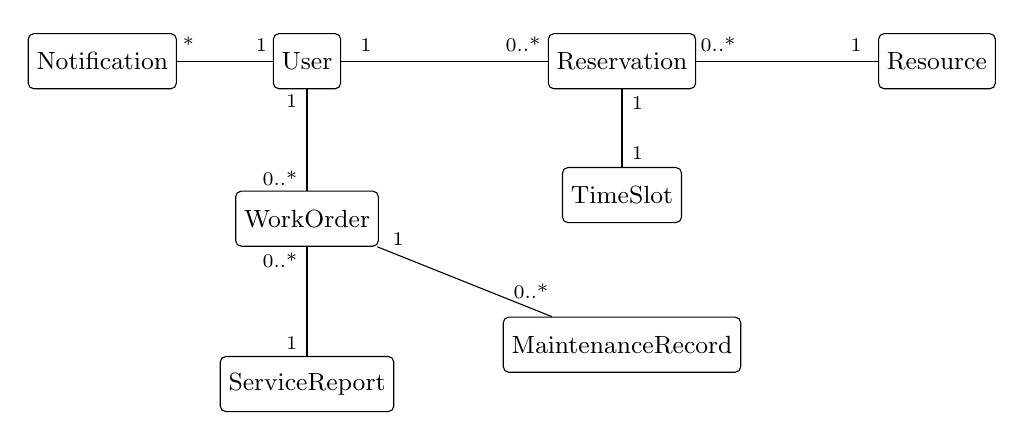
\begin{tikzpicture}[node distance=15mm and 20mm]
\node[umlbox] (notification) at (-2.6,2.7) {Notification};
\node[umlbox] (user) at (0,2.7) {User};
\node[umlbox] (reservation) at (4,2.7) {Reservation};
\node[umlbox] (resource) at (8,2.7) {Resource};
\node[umlbox] (timeslot) at (4,1.0) {TimeSlot};
\node[umlbox] (workorder) at (0,0.7) {WorkOrder};
\node[umlbox] (maintenance) at (4,-0.9) {MaintenanceRecord};
\node[umlbox] (report) at (0,-1.4) {ServiceReport};
\draw (user) -- node[above,pos=0.12,font=\scriptsize] {1} node[above,pos=0.88,font=\scriptsize] {0..*} (reservation);
\draw (resource) -- node[above,pos=0.12,font=\scriptsize] {1} node[above,pos=0.88,font=\scriptsize] {0..*} (reservation);
\draw (reservation) -- node[right,pos=0.18,font=\scriptsize] {1} node[right,pos=0.82,font=\scriptsize] {1} (timeslot);
\draw (user) -- node[left,pos=0.12,font=\scriptsize] {1} node[left,pos=0.88,font=\scriptsize] {0..*} (workorder);
\draw (workorder) -- node[above,pos=0.12,font=\scriptsize] {1} node[above,pos=0.88,font=\scriptsize] {0..*} (maintenance);
\draw (notification) -- node[above,pos=0.12,font=\scriptsize] {*} node[above,pos=0.88,font=\scriptsize] {1} (user);
\draw (report) -- node[left,pos=0.12,font=\scriptsize] {1} node[left,pos=0.88,font=\scriptsize] {0..*} (workorder);
\end{tikzpicture}}
\end{center}


系统顺序图：

\begin{center}
\resizebox{0.95\linewidth}{!}{%
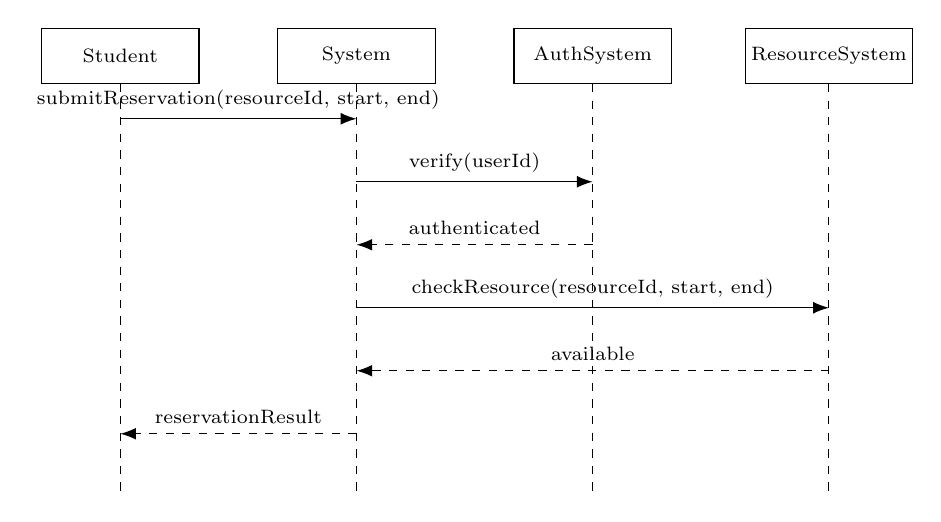
\begin{tikzpicture}
\node[umllifeline] (student) at (0,0) {Student};
\node[umllifeline] (system) at (3,0) {System};
\node[umllifeline] (auth) at (6,0) {AuthSystem};
\node[umllifeline] (resourceSystem) at (9,0) {ResourceSystem};
\foreach \p in {student,system,auth,resourceSystem} {
  \draw[dashed] (\p.south) -- ++(0,-5.2);
}
\draw[umlmsg] (0,-0.8) -- node[above,font=\scriptsize] {submitReservation(resourceId, start, end)} (3,-0.8);
\draw[umlmsg] (3,-1.6) -- node[above,font=\scriptsize] {verify(userId)} (6,-1.6);
\draw[umlreturn] (6,-2.4) -- node[above,font=\scriptsize] {authenticated} (3,-2.4);
\draw[umlmsg] (3,-3.2) -- node[above,font=\scriptsize] {checkResource(resourceId, start, end)} (9,-3.2);
\draw[umlreturn] (9,-4.0) -- node[above,font=\scriptsize] {available} (3,-4.0);
\draw[umlreturn] (3,-4.8) -- node[above,font=\scriptsize] {reservationResult} (0,-4.8);
\end{tikzpicture}}
\end{center}


评分点：


\begin{quote}
\footnotesize
\begin{verbatim}
概念类图只写问题域概念，不写 Controller、Service、Repository。
系统顺序图把系统看成黑盒，只写参与者、系统和外部系统。
\end{verbatim}
\end{quote}


\subsubsection*{四、体系结构设计题答案}


物理包图：

\begin{center}
\resizebox{0.95\linewidth}{!}{%
\begin{tikzpicture}[node distance=22mm]
\node[packagebox] (client) {
\begin{tabular}{c}
\textbf{客户端 / 浏览器}\\
html\\
css\\
javascript\\
presentation
\end{tabular}};
\node[packagebox, right=26mm of client] (server) {
\begin{tabular}{c}
\textbf{服务器端}\\
controller/api\\
service\\
repository\\
domain/entity\\
modules\\
reservation \quad resource \quad workorder\\
notification \quad user\\
database
\end{tabular}};
\draw[umlmsg] (client.east) -- node[above,align=center,font=\small] {HTTP + REST API + JSON} (server.west);
\end{tikzpicture}}
\end{center}


接口代码：


\begin{quote}
\footnotesize
\begin{verbatim}
package edu.nju.service;

public interface ReservationService {
    ReservationResult reserve(ReservationCommand command);
}

package edu.nju.repository;

public interface ResourceRepository {
    Optional<Resource> findById(Long resourceId);
    void save(Resource resource);
}

package edu.nju.repository;

public interface ReservationRepository {
    void save(Reservation reservation);
    List<Reservation> findByResourceAndTimeRange(Long resourceId, TimeRange range);
}

package edu.nju.controller;

@RestController
@RequestMapping("/api/reservations")
public class ReservationController {
    private final ReservationService reservationService;

    public ReservationController(ReservationService reservationService) {
        this.reservationService = reservationService;
    }

    @PostMapping
    public ReservationResult reserve(@RequestBody ReservationCommand command) {
        return reservationService.reserve(command);
    }
}
\end{verbatim}
\end{quote}


\subsubsection*{五、详细设计题答案}


详细顺序图：

\begin{center}
\resizebox{\linewidth}{!}{%
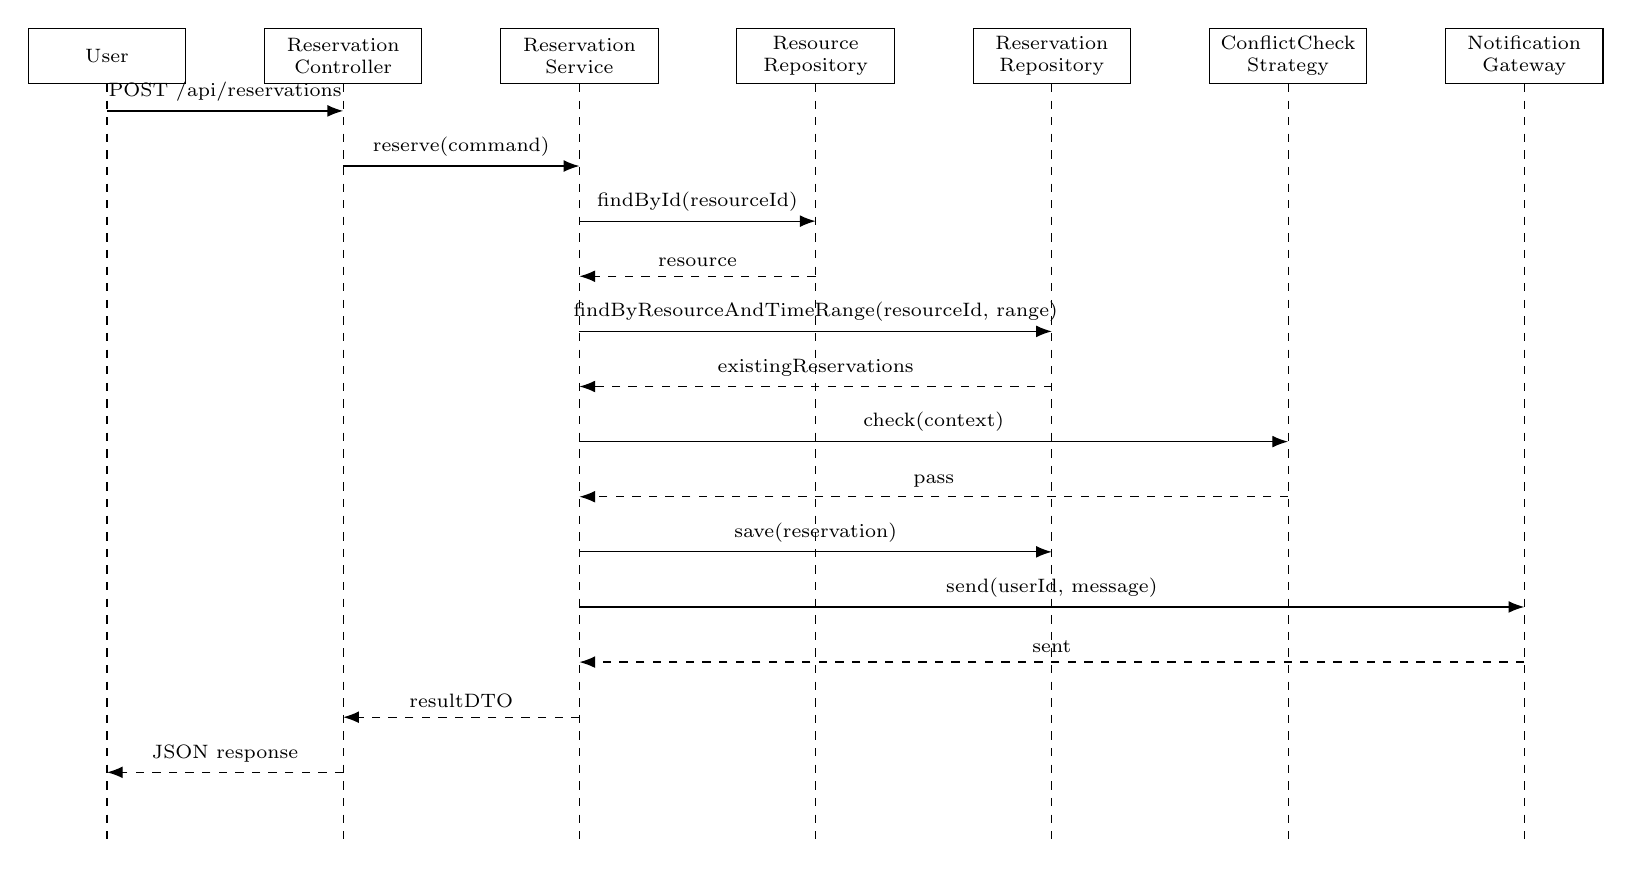
\begin{tikzpicture}
\node[umllifeline] (user) at (0,0) {User};
\node[umllifeline] (controller) at (3,0) {Reservation\\Controller};
\node[umllifeline] (service) at (6,0) {Reservation\\Service};
\node[umllifeline] (resourceRepo) at (9,0) {Resource\\Repository};
\node[umllifeline] (reservationRepo) at (12,0) {Reservation\\Repository};
\node[umllifeline] (strategy) at (15,0) {ConflictCheck\\Strategy};
\node[umllifeline] (notification) at (18,0) {Notification\\Gateway};
\foreach \p in {user,controller,service,resourceRepo,reservationRepo,strategy,notification} {
  \draw[dashed] (\p.south) -- ++(0,-9.6);
}
\draw[umlmsg] (0,-0.7) -- node[above,font=\scriptsize] {POST /api/reservations} (3,-0.7);
\draw[umlmsg] (3,-1.4) -- node[above,font=\scriptsize] {reserve(command)} (6,-1.4);
\draw[umlmsg] (6,-2.1) -- node[above,font=\scriptsize] {findById(resourceId)} (9,-2.1);
\draw[umlreturn] (9,-2.8) -- node[above,font=\scriptsize] {resource} (6,-2.8);
\draw[umlmsg] (6,-3.5) -- node[above,font=\scriptsize] {findByResourceAndTimeRange(resourceId, range)} (12,-3.5);
\draw[umlreturn] (12,-4.2) -- node[above,font=\scriptsize] {existingReservations} (6,-4.2);
\draw[umlmsg] (6,-4.9) -- node[above,font=\scriptsize] {check(context)} (15,-4.9);
\draw[umlreturn] (15,-5.6) -- node[above,font=\scriptsize] {pass} (6,-5.6);
\draw[umlmsg] (6,-6.3) -- node[above,font=\scriptsize] {save(reservation)} (12,-6.3);
\draw[umlmsg] (6,-7.0) -- node[above,font=\scriptsize] {send(userId, message)} (18,-7.0);
\draw[umlreturn] (18,-7.7) -- node[above,font=\scriptsize] {sent} (6,-7.7);
\draw[umlreturn] (6,-8.4) -- node[above,font=\scriptsize] {resultDTO} (3,-8.4);
\draw[umlreturn] (3,-9.1) -- node[above,font=\scriptsize] {JSON response} (0,-9.1);
\end{tikzpicture}}
\end{center}


控制风格：


\begin{quote}
\footnotesize
\begin{verbatim}
集中式控制：少数控制对象掌握大部分流程，决策位置清楚，但控制器容易膨胀。
委托式控制：入口对象保留主流程，把专业子任务委托给 Service、领域对象、策略对象和 Repository。
分散式控制：多个对象共同推进流程，单对象轻，但控制流难追踪。
\end{verbatim}
\end{quote}


本场景采用委托式控制：


\begin{quote}
\footnotesize
\begin{verbatim}
Controller 只处理请求和响应。
Service 组织业务流程和事务。
Repository 隐藏持久化。
Strategy 处理冲突检测变化点。
NotificationGateway 隐藏外部消息服务。
\end{verbatim}
\end{quote}


\subsubsection*{六、模块化与信息隐藏题答案}


问题：


\begin{quote}
\footnotesize
\begin{verbatim}
1. 包之间互相直接访问内部对象，形成高访问耦合和循环依赖。
2. 多个包共享可变全局配置，形成公共耦合。
3. 业务规则、通知、资源状态和用户权限混在不同包中，职责边界不清。
4. 内部数据结构暴露后，字段修改会传播到多个包。
\end{verbatim}
\end{quote}


违反原则：


\begin{quote}
\footnotesize
\begin{verbatim}
信息隐藏：内部数据结构和变化点没有被封装。
DIP：高层业务直接依赖低层实现对象。
SRP：包和类存在多个变化理由。
Law of Demeter：跨对象链式访问过多。
ADP：包依赖关系中存在环。
\end{verbatim}
\end{quote}


改进：


\begin{quote}
\footnotesize
\begin{verbatim}
reservation 包只暴露 ReservationService。
resource 包只暴露 ResourceQueryService 或 ResourceRepository 接口。
notification 包只暴露 NotificationGateway。
user 包只暴露 UserService 或 AuthGateway。
公共配置改为不可变配置对象，通过构造器注入。
跨包传递 DTO 或领域接口，不返回内部可变集合。
\end{verbatim}
\end{quote}


\subsubsection*{七、设计模式题答案}


Strategy：

\begin{center}
\resizebox{0.95\linewidth}{!}{%
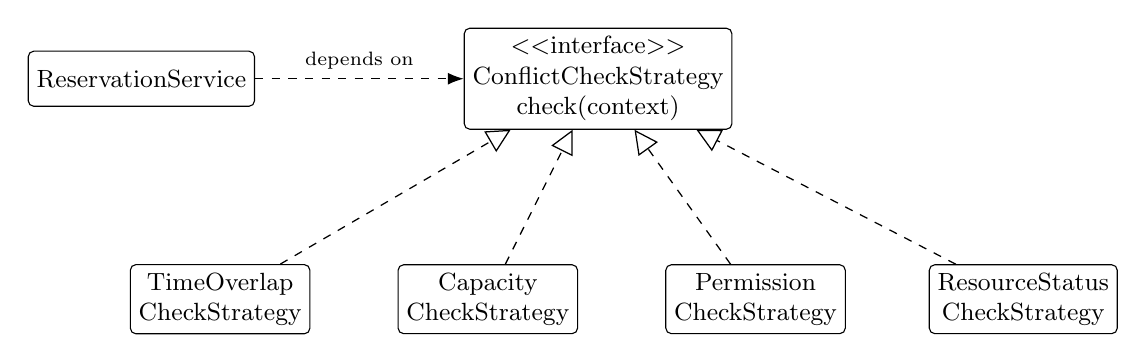
\begin{tikzpicture}[node distance=12mm and 14mm]
\node[umlbox] (service) at (0,1.8) {ReservationService};
\node[umlbox] (strategy) at (5.8,1.8) {\textless\textless interface\textgreater\textgreater\\ConflictCheckStrategy\\check(context)};
\node[umlbox] (time) at (1.0,-1.0) {TimeOverlap\\CheckStrategy};
\node[umlbox] (capacity) at (4.4,-1.0) {Capacity\\CheckStrategy};
\node[umlbox] (permission) at (7.8,-1.0) {Permission\\CheckStrategy};
\node[umlbox] (status) at (11.2,-1.0) {ResourceStatus\\CheckStrategy};
\draw[umlmsg,dashed] (service.east) -- node[above,font=\scriptsize] {depends on} (strategy.west);
\draw[umlrealize] (time) -- (strategy);
\draw[umlrealize] (capacity) -- (strategy);
\draw[umlrealize] (permission) -- (strategy);
\draw[umlrealize] (status) -- (strategy);
\end{tikzpicture}}
\end{center}

ReservationService 依赖 ConflictCheckStrategy 接口。新增冲突规则时新增策略类，不修改主流程。


Abstract Factory / DAO Factory：

\begin{center}
\resizebox{0.95\linewidth}{!}{%
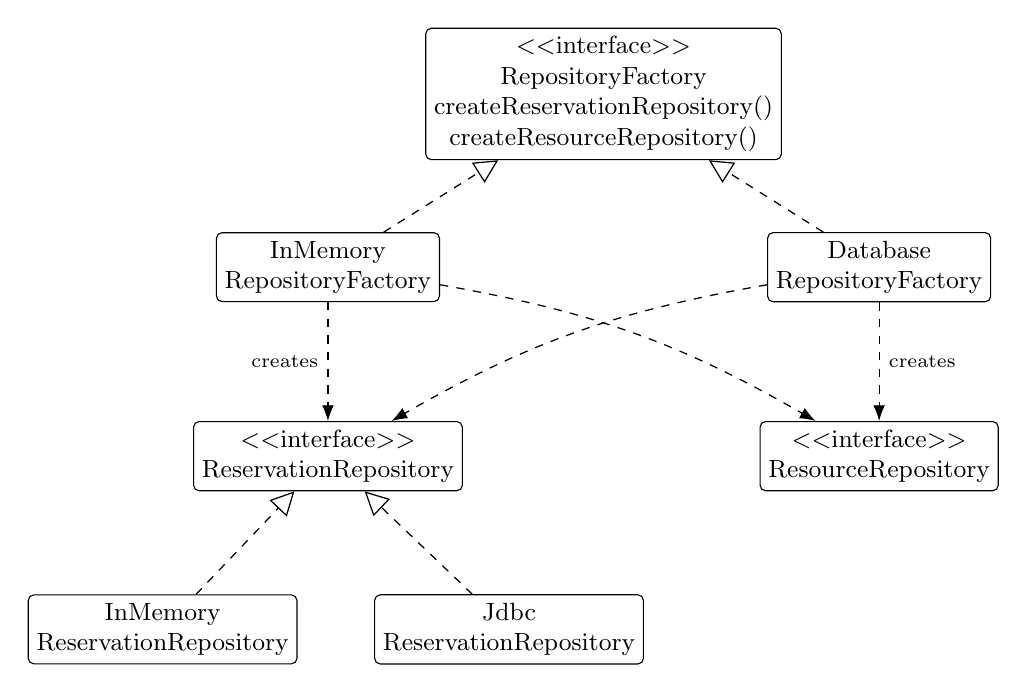
\begin{tikzpicture}[node distance=12mm and 16mm]
\node[umlbox] (factory) at (4,2.2) {\textless\textless interface\textgreater\textgreater\\RepositoryFactory\\createReservationRepository()\\createResourceRepository()};
\node[umlbox] (memFactory) at (0.5,0) {InMemory\\RepositoryFactory};
\node[umlbox] (dbFactory) at (7.5,0) {Database\\RepositoryFactory};
\node[umlbox] (reservationRepo) at (0.5,-2.4) {\textless\textless interface\textgreater\textgreater\\ReservationRepository};
\node[umlbox] (resourceRepo) at (7.5,-2.4) {\textless\textless interface\textgreater\textgreater\\ResourceRepository};
\node[umlbox] (memReservation) at (-1.6,-4.6) {InMemory\\ReservationRepository};
\node[umlbox] (jdbcReservation) at (2.8,-4.6) {Jdbc\\ReservationRepository};
\draw[umlrealize] (memFactory) -- (factory);
\draw[umlrealize] (dbFactory) -- (factory);
\draw[umlmsg,dashed] (memFactory) -- node[left,font=\scriptsize] {creates} (reservationRepo);
\draw[umlmsg,dashed] (memFactory) to[bend left=10] (resourceRepo);
\draw[umlmsg,dashed] (dbFactory) to[bend right=10] (reservationRepo);
\draw[umlmsg,dashed] (dbFactory) -- node[right,font=\scriptsize] {creates} (resourceRepo);
\draw[umlrealize] (memReservation) -- (reservationRepo);
\draw[umlrealize] (jdbcReservation) -- (reservationRepo);
\end{tikzpicture}}
\end{center}


原则：


\begin{quote}
\footnotesize
\begin{verbatim}
OCP：新增规则或数据访问实现时扩展新类。
DIP：Service 依赖接口，不依赖具体实现。
SRP：每个策略只负责一种冲突检测。
信息隐藏：Repository 隐藏存储细节。
\end{verbatim}
\end{quote}


\subsubsection*{八、软件构造题答案}


问题：


\begin{quote}
\footnotesize
\begin{verbatim}
1. 条件表达式过长，可读性差。
2. status == 1 是魔法数字。
3. 方法同时负责校验、查询、保存和通知，违反 SRP。
4. 直接访问 dao 和 msg，依赖具体实现。
5. 失败时只返回 false，缺少明确失败原因。
6. 没有异常处理、事务边界和测试切入点。
\end{verbatim}
\end{quote}


重构方向：


\begin{quote}
\footnotesize
\begin{verbatim}
提取输入校验方法。
用枚举表达资源状态。
用 Strategy 或规则列表表达预约规则。
Service 依赖 Repository 和 Gateway 接口。
返回 ReservationResult，包含成功状态和失败原因。
用 Mock 替代外部依赖进行单元测试。
\end{verbatim}
\end{quote}


代码骨架：


\begin{quote}
\footnotesize
\begin{verbatim}
public class ReservationService {
    private final ResourceRepository resourceRepository;
    private final ReservationRepository reservationRepository;
    private final List<ReservationRule> rules;
    private final NotificationGateway notificationGateway;

    public ReservationResult reserve(ReservationCommand command) {
        validate(command);
        Resource resource = resourceRepository.findById(command.resourceId())
                .orElseThrow(() -> new BusinessException("resource not found"));
        ReservationContext context = ReservationContext.of(command, resource);

        for (ReservationRule rule : rules) {
            RuleResult result = rule.check(context);
            if (!result.pass()) {
                return ReservationResult.fail(result.reason());
            }
        }

        Reservation reservation = Reservation.create(command);
        reservationRepository.save(reservation);
        notificationGateway.send(command.userId(), "reservation accepted");
        return ReservationResult.success(reservation.id());
    }
}
\end{verbatim}
\end{quote}


\subsubsection*{九、测试题答案}


圈复杂度：


\begin{quote}
\footnotesize
\begin{verbatim}
V(G) = 判定节点数 + 1。
若 C1、C2、C3、C4 分别作为 4 个独立判定，则 V(G)=5。
若实现为一个复合 if，按题目要求拆分基本条件进行条件覆盖。
\end{verbatim}
\end{quote}


条件覆盖测试：


\begin{quote}
\footnotesize
\begin{verbatim}
T1: C1=T, C2=T, C3=T, C4=T -> A1 保存预约。
T2: C1=F, C2=T, C3=T, C4=T -> A2 返回未登录。
T3: C1=T, C2=F, C3=T, C4=T -> A2 返回资源不可预约。
T4: C1=T, C2=T, C3=F, C4=T -> A2 返回时间段非法。
T5: C1=T, C2=T, C3=T, C4=F -> A2 返回容量已满。
\end{verbatim}
\end{quote}


Mock：


\begin{quote}
\footnotesize
\begin{verbatim}
用 Mock NotificationGateway 替代真实消息服务。
成功路径断言 send(userId, message) 被调用一次。
失败路径断言 send 不被调用。
当 Mock 抛出异常时，断言 Service 返回失败或触发回滚逻辑。
\end{verbatim}
\end{quote}


\subsubsection*{十、人机交互题答案}


\begin{quote}
\footnotesize
\begin{verbatim}
系统状态可见：提交中、审核中、预约成功、冲突失败必须明确显示。
错误预防：非法时间段、已满资源和权限不足应在提交前提示。
识别优于回忆：日历直接显示可预约时段，减少用户记忆资源编号。
一致性和标准：按钮位置、颜色、术语在预约、工单和报表页面保持一致。
用户控制和自由：提供取消预约、修改时间段、返回列表和重新提交入口。
Fitts 定律：高频按钮靠近主要操作区域，按钮尺寸足够大。
美学和极简：默认显示关键任务信息，历史记录和高级筛选折叠。
帮助用户恢复错误：冲突提示应给出可选时间段，而不是只显示失败。
\end{verbatim}
\end{quote}


\section{补充模拟卷 01：旧题简答与过程模型补缺}


\subsection{A 卷题目}


\subsubsection*{一、软件工程发展、团队与质量保障（20 分）}


\begin{enumerate}
\item 概括 1950s 到 2000s 软件工程发展的阶段特点。
\item 写出三种团队结构。
\item 结合项目说明质量保障活动覆盖哪些阶段。
\end{enumerate}


\subsubsection*{二、配置管理与持续集成（20 分）}


\begin{enumerate}
\item 写出软件配置管理的活动。
\item 说明配置项和基线。
\item 解释 CI/CD 和配置管理的关系。
\end{enumerate}


\subsubsection*{三、需求规格说明（20 分）}


\begin{enumerate}
\item 说明为什么需要建立需求规格说明。
\item 写出需求规格说明常见书写要求。
\item 修改下面需求中的问题：
\end{enumerate}


\begin{quote}
\footnotesize
\begin{verbatim}
系统应该尽快处理预约，并且界面要非常友好。
程序调用 ReservationService 的 check 方法验证所有参数。
\end{verbatim}
\end{quote}


\subsubsection*{四、过程模型比较（20 分）}


比较：


\begin{quote}
\footnotesize
\begin{verbatim}
Build-and-Fix
Waterfall
Incremental Iteration
Evolutionary Model
Prototype Model
Spiral Model
\end{verbatim}
\end{quote}


要求写出核心思想、适用场景和主要风险。


\subsubsection*{五、维护、文档、逆向工程与再工程（20 分）}


\begin{enumerate}
\item 说明软件维护的重要性。
\item 区分用户文档和系统文档。
\item 区分逆向工程和再工程。
\end{enumerate}


\subsection{B 简明答案}


\subsubsection*{一、软件工程发展、团队与质量保障答案}


阶段特点：


\begin{quote}
\footnotesize
\begin{verbatim}
1950s：科学计算，以机器为中心编程。
1960s：业务应用和事务处理增长，软件不同于硬件的特征凸显。
1970s：结构化方法和瀑布模型发展，强调规则和纪律。
1980s：追求生产力，结构化方法和面向对象方法广泛应用，重视过程。
1990s：企业级大规模系统和 Web 应用出现，强调快速开发、可变更性和用户价值。
2000s：大众 Web 产品和大规模 Web 应用增长，强调快速迭代、创新和用户反馈。
\end{verbatim}
\end{quote}


团队结构：


\begin{quote}
\footnotesize
\begin{verbatim}
主程序员团队。
民主团队。
开放团队。
\end{verbatim}
\end{quote}


质量保障：


\begin{quote}
\footnotesize
\begin{verbatim}
需求阶段：需求评审、需求度量。
体系结构阶段：架构评审、集成测试策略。
详细设计阶段：设计评审、设计度量、集成测试准备。
构造阶段：代码评审、代码度量、单元测试、持续集成。
测试阶段：测试执行、缺陷度量、覆盖率分析、回归测试。
\end{verbatim}
\end{quote}


\subsubsection*{二、配置管理与持续集成答案}


SCM 活动：


\begin{quote}
\footnotesize
\begin{verbatim}
配置项识别。
版本管理。
变更控制。
配置审计。
状态报告。
软件发布管理。
\end{verbatim}
\end{quote}


配置项和基线：


\begin{quote}
\footnotesize
\begin{verbatim}
配置项是纳入配置管理的制品，包括需求文档、设计文档、
源代码、测试脚本、配置文件、数据库脚本和部署脚本。
基线是经过评审和批准的规格或产品版本，后续变更必须经过正式变更控制。
\end{verbatim}
\end{quote}


CI/CD：


\begin{quote}
\footnotesize
\begin{verbatim}
CI 通过自动构建、自动测试和静态检查保证主干持续可集成。
CD 通过自动或半自动发布保证发布过程可重复、可审计、可回滚。
它们把配置管理中的构建、版本、发布和验证活动自动化。
\end{verbatim}
\end{quote}


\subsubsection*{三、需求规格说明答案}


必要性：


\begin{quote}
\footnotesize
\begin{verbatim}
1. 方便交流：把问题域理解和系统解决方案文档化。
2. 建立基线：方便任务分配、进度计划、跟踪和度量。
3. 支持验证：需求可以被评审、测试和追踪。
4. 支持变更管理：变更可以分析影响范围。
\end{verbatim}
\end{quote}


书写要求：


\begin{quote}
\footnotesize
\begin{verbatim}
使用用户术语。
简洁、精确、易读、易修改。
可验证。
可实现。
避免模糊形容词和程度词。
避免把内部类名、方法名、参数名写成用户需求。
\end{verbatim}
\end{quote}


修改：


\begin{quote}
\footnotesize
\begin{verbatim}
原句问题：
“尽快”“非常友好”不可验证。
“程序调用 ReservationService 的 check 方法”使用实现术语。

改写：
系统应在用户提交预约请求后 2 秒内返回处理结果。
系统应在预约时间冲突时显示冲突原因和至少一个可选时间段。
系统应校验预约请求中的用户身份、资源状态、时间段和容量限制。
\end{verbatim}
\end{quote}


\subsubsection*{四、过程模型比较答案}


\begin{quote}
\footnotesize
\begin{verbatim}
Build-and-Fix：
无明确过程，直接构建再修补。适合极小实验程序。风险是结构退化、缺少文档、难测试、难维护。

Waterfall：
需求、设计、实现、测试、交付顺序推进。
适合需求稳定、合同边界清楚的项目。
风险是反馈晚，早期需求错误会传递到后期。

Incremental Iteration：
按功能增量分批交付，每轮迭代完善。
适合核心需求清楚、功能可拆分的系统。
风险是需要稳定架构和增量规划。

Evolutionary Model：
交付初始版本后根据反馈持续演化。适合需求变化频繁的系统。风险是范围和进度难控制。

Prototype Model：
用原型澄清界面、流程和规则。适合需求表达不清的项目。风险是把抛弃式原型直接当最终产品。

Spiral Model：
风险驱动，每轮包括目标设定、风险分析、开发验证和计划下一轮。
适合大型高风险项目。
风险是对风险识别能力要求高。
\end{verbatim}
\end{quote}


\subsubsection*{五、维护、文档、逆向工程与再工程答案}


维护：


\begin{quote}
\footnotesize
\begin{verbatim}
软件维护是在交付后修改软件系统或部件，以修正缺陷、改进性能或适应环境变化。
软件不会物理磨损，但会因需求、环境、依赖和业务变化而持续需要修改。
\end{verbatim}
\end{quote}


文档：


\begin{quote}
\footnotesize
\begin{verbatim}
用户文档面向最终用户，说明安装、登录、导航、操作步骤、输入格式、错误恢复和常见问题。
系统文档面向维护和运维人员，说明软硬件配置、网络、安全、备份、部署、故障处理和部件替换。
\end{verbatim}
\end{quote}


逆向工程与再工程：


\begin{quote}
\footnotesize
\begin{verbatim}
逆向工程从已有系统恢复部件、交互、需求和设计，核心是理解和抽象。
再工程在理解旧系统基础上重构、迁移或重新实现，目标是改善结构、质量、可维护性和可演化性。
\end{verbatim}
\end{quote}


\section{补充模拟卷 02：需求建模与图形题补缺}


\subsection{A 卷题目}


\subsubsection*{一、图书馆系统用例建模（20 分）}


场景：图书馆系统支持读者查询图书、借书、还书、预约图书；馆员办理借还；管理员检查超期未还并打印分类书目。


完成：


\begin{enumerate}
\item 写出建模步骤。
\item 写出参与者和用例。
\item 标注一组 \texttt{include} 和一组 \texttt{extend}。
\end{enumerate}


\subsubsection*{二、ATM 领域模型（20 分）}


场景：ATM 通过屏幕、键盘、读卡器、存款口、打印机与客户交互。客户可存款、取款、查询余额。账户更新由银行账户系统完成，安全系统负责 PIN 验证。


完成概念类图。


\subsubsection*{三、状态图与系统顺序图（20 分）}


针对维修工单：


\begin{quote}
\footnotesize
\begin{verbatim}
提交 -> 待审核 -> 已分派 -> 处理中 -> 已完成 -> 已关闭
\end{verbatim}
\end{quote}


完成：


\begin{enumerate}
\item 写出状态、事件和转换。
\item 写出“提交维修工单”的系统顺序图。
\end{enumerate}


\subsubsection*{四、需求错误识别与功能测试（20 分）}


需求片段：


\begin{quote}
\footnotesize
\begin{verbatim}
系统应该拥有现代化界面。
用户点击按钮以后系统调用 WorkOrderDao.insert。
管理员能很方便地处理所有异常工单。
\end{verbatim}
\end{quote}


完成：


\begin{enumerate}
\item 指出问题。
\item 改写为可验证需求。
\item 为“提交维修工单”设计功能测试用例。
\end{enumerate}


\subsubsection*{五、概念类图、系统顺序图和详细顺序图区别（20 分）}


说明三者的目的、图中对象、考试作答边界。


\subsection{B 简明答案}


\subsubsection*{一、图书馆系统用例建模答案}


建模步骤：


\begin{quote}
\footnotesize
\begin{verbatim}
1. 确定系统边界。
2. 找参与者。
3. 找有业务价值的用例。
4. 合并过细操作。
5. 标注 include、extend 和泛化。
\end{verbatim}
\end{quote}


用例图：

\begin{center}
\resizebox{0.95\linewidth}{!}{%
\begin{tikzpicture}
\node[usecase] (query) at (2.0,2.0) {查询图书};
\node[usecase] (borrow) at (4.8,1.0) {借出图书};
\node[usecase] (return) at (2.0,-0.2) {归还图书};
\node[usecase] (reserve) at (4.8,2.4) {预约图书};
\node[usecase] (overdue) at (6.9,-0.5) {检查超期未还};
\node[usecase] (print) at (6.9,-2.0) {打印分类书目};
\node[usecase] (download) at (4.0,-2.5) {下载读者信息};
\node[draw, rounded corners=2pt, fit=(query)(borrow)(return)(reserve)(overdue)(print)(download), inner xsep=8mm, inner ysep=7mm, label={[font=\small]above:图书馆系统}] (systemBoundary) {};
\node[align=center] (reader) at (-1.2,1.4) {\umlactor{读者}};
\node[align=center] (librarian) at (-1.2,-0.7) {\umlactor{馆员}};
\node[align=center] (admin) at (10.2,-0.5) {\umlactor{管理员}};
\node[align=center] (external) at (10.2,-2.5) {\umlactor{外部大学数据库}};
\draw (reader) -- (query);
\draw (reader) -- (reserve);
\draw (librarian) -- (borrow);
\draw (librarian) -- (return);
\draw (admin) -- (overdue);
\draw (admin) -- (print);
\draw (external) -- (download);
\draw[umlmsg,dashed] (borrow) -- node[above,font=\scriptsize] {\textless\textless include\textgreater\textgreater} (query);
\draw[umlmsg,dashed] (reserve) -- node[above,font=\scriptsize] {\textless\textless extend\textgreater\textgreater} (query);
\end{tikzpicture}}
\end{center}


\subsubsection*{二、ATM 领域模型答案}


领域类图：

\begin{center}
\resizebox{\linewidth}{!}{%
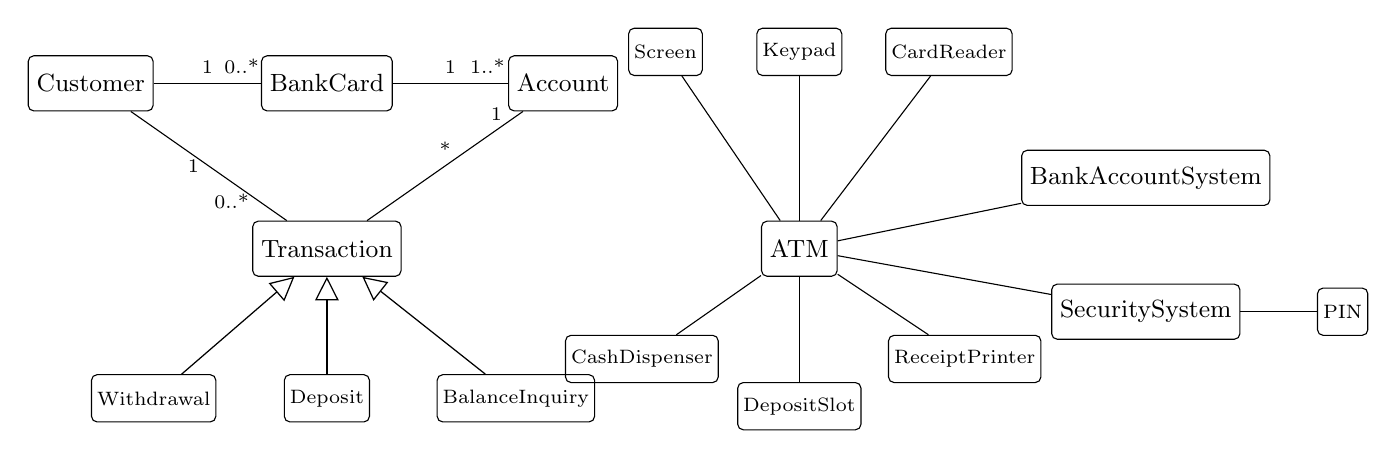
\begin{tikzpicture}
\node[umlbox] (customer) at (0,2.3) {Customer};
\node[umlbox] (card) at (3.0,2.3) {BankCard};
\node[umlbox] (account) at (6.0,2.3) {Account};
\node[umlbox] (transaction) at (3.0,0.2) {Transaction};
\node[umlsmallbox] (withdrawal) at (0.8,-1.7) {Withdrawal};
\node[umlsmallbox] (deposit) at (3.0,-1.7) {Deposit};
\node[umlsmallbox] (balance) at (5.4,-1.7) {BalanceInquiry};
\node[umlbox] (atm) at (9.0,0.2) {ATM};
\node[umlsmallbox] (screen) at (7.3,2.7) {Screen};
\node[umlsmallbox] (keypad) at (9.0,2.7) {Keypad};
\node[umlsmallbox] (reader) at (10.9,2.7) {CardReader};
\node[umlsmallbox] (cash) at (7.0,-1.2) {CashDispenser};
\node[umlsmallbox] (slot) at (9.0,-1.8) {DepositSlot};
\node[umlsmallbox] (printer) at (11.1,-1.2) {ReceiptPrinter};
\node[umlbox] (bankSystem) at (13.4,1.1) {BankAccountSystem};
\node[umlbox] (security) at (13.4,-0.6) {SecuritySystem};
\node[umlsmallbox] (pin) at (15.9,-0.6) {PIN};
\draw (customer) -- node[above,font=\scriptsize] {1} node[above,pos=0.82,font=\scriptsize] {0..*} (card);
\draw (card) -- node[above,font=\scriptsize] {1} node[above,pos=0.82,font=\scriptsize] {1..*} (account);
\draw (customer) -- node[left,font=\scriptsize] {1} node[left,pos=0.82,font=\scriptsize] {0..*} (transaction);
\draw (transaction) -- node[above,font=\scriptsize] {*} node[above,pos=0.83,font=\scriptsize] {1} (account);
\draw[umlinherit] (withdrawal) -- (transaction);
\draw[umlinherit] (deposit) -- (transaction);
\draw[umlinherit] (balance) -- (transaction);
\foreach \device in {screen,keypad,reader,cash,slot,printer} {
  \draw (atm) -- (\device);
}
\draw (atm) -- (bankSystem);
\draw (atm) -- (security);
\draw (security) -- (pin);
\end{tikzpicture}}
\end{center}


评分点：


\begin{quote}
\footnotesize
\begin{verbatim}
领域模型写业务概念和设备概念，不写 Controller、Service、DAO。
交易类型用继承表达。
外部账户系统和安全系统作为外部系统概念。
\end{verbatim}
\end{quote}


\subsubsection*{三、状态图与系统顺序图答案}


状态转换：

\begin{center}
\resizebox{0.9\linewidth}{!}{%
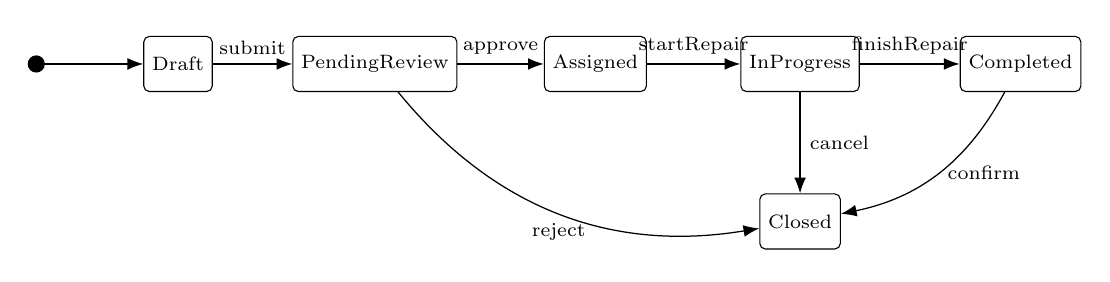
\begin{tikzpicture}[node distance=13mm and 17mm]
\node[circle, fill=black, inner sep=2.2pt] (start) at (-1.3,0) {};
\node[statebox] (draft) at (0.5,0) {Draft};
\node[statebox] (pending) at (3.0,0) {PendingReview};
\node[statebox] (assigned) at (5.8,0) {Assigned};
\node[statebox] (progress) at (8.4,0) {InProgress};
\node[statebox] (completed) at (11.2,0) {Completed};
\node[statebox] (closed) at (8.4,-2.0) {Closed};
\draw[umlmsg] (start) -- (draft);
\draw[umlmsg] (draft) -- node[above,font=\scriptsize] {submit} (pending);
\draw[umlmsg] (pending) -- node[above,font=\scriptsize] {approve} (assigned);
\draw[umlmsg] (pending) to[bend right=30] node[below,font=\scriptsize] {reject} (closed);
\draw[umlmsg] (assigned) -- node[above,font=\scriptsize] {startRepair} (progress);
\draw[umlmsg] (progress) -- node[above,font=\scriptsize] {finishRepair} (completed);
\draw[umlmsg] (completed) to[bend left=25] node[right,font=\scriptsize] {confirm} (closed);
\draw[umlmsg] (progress) -- node[right,font=\scriptsize] {cancel} (closed);
\end{tikzpicture}}
\end{center}


系统顺序图：

\begin{center}
\resizebox{0.95\linewidth}{!}{%
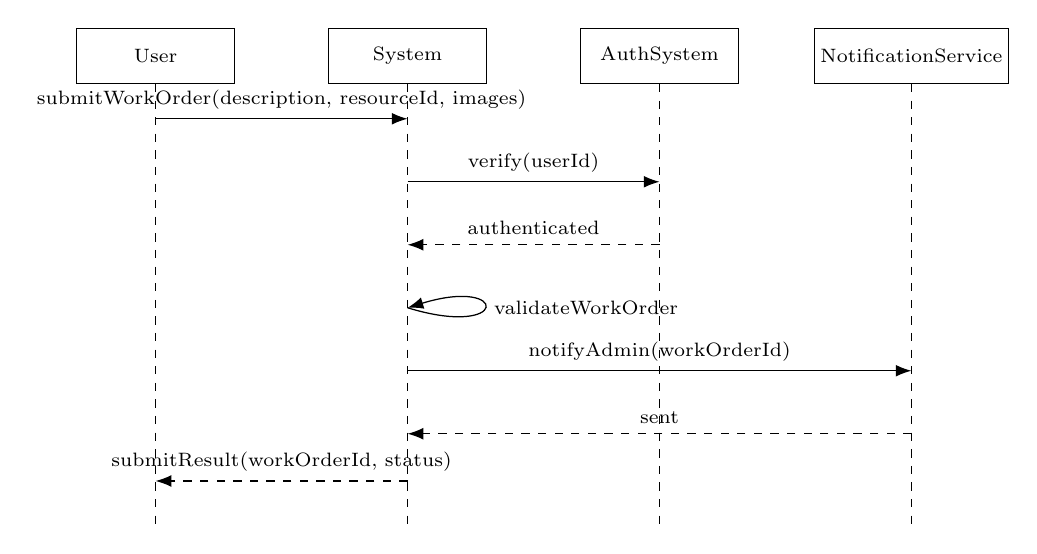
\begin{tikzpicture}
\node[umllifeline] (user) at (0,0) {User};
\node[umllifeline] (system) at (3.2,0) {System};
\node[umllifeline] (auth) at (6.4,0) {AuthSystem};
\node[umllifeline] (notification) at (9.6,0) {NotificationService};
\foreach \p in {user,system,auth,notification} {
  \draw[dashed] (\p.south) -- ++(0,-5.6);
}
\draw[umlmsg] (0,-0.8) -- node[above,font=\scriptsize] {submitWorkOrder(description, resourceId, images)} (3.2,-0.8);
\draw[umlmsg] (3.2,-1.6) -- node[above,font=\scriptsize] {verify(userId)} (6.4,-1.6);
\draw[umlreturn] (6.4,-2.4) -- node[above,font=\scriptsize] {authenticated} (3.2,-2.4);
\draw[umlmsg] (3.2,-3.2) .. controls (4.5,-3.6) and (4.5,-2.8) .. node[right,font=\scriptsize] {validateWorkOrder} (3.2,-3.2);
\draw[umlmsg] (3.2,-4.0) -- node[above,font=\scriptsize] {notifyAdmin(workOrderId)} (9.6,-4.0);
\draw[umlreturn] (9.6,-4.8) -- node[above,font=\scriptsize] {sent} (3.2,-4.8);
\draw[umlreturn] (3.2,-5.4) -- node[above,font=\scriptsize] {submitResult(workOrderId, status)} (0,-5.4);
\end{tikzpicture}}
\end{center}


\subsubsection*{四、需求错误识别与功能测试答案}


问题：


\begin{quote}
\footnotesize
\begin{verbatim}
“现代化”“很方便”不可验证。
“调用 WorkOrderDao.insert”使用实现术语。
“所有异常工单”范围过大，缺少异常类型和处理规则。
\end{verbatim}
\end{quote}


改写：


\begin{quote}
\footnotesize
\begin{verbatim}
系统应在用户提交维修工单后 2 秒内返回工单编号和初始状态。
系统应要求用户填写资源编号、故障描述和联系方式，缺失任一必填项时拒绝提交并显示字段级错误信息。
管理员应能按工单状态、资源编号和提交时间筛选工单。
系统应支持管理员将待审核工单分派给维修人员，并记录分派时间和处理人。
\end{verbatim}
\end{quote}


功能测试用例：


\begin{quote}
\footnotesize
\begin{verbatim}
T1: 必填项完整，资源存在 -> 提交成功，返回工单编号和待审核状态。
T2: 故障描述为空 -> 提交失败，提示故障描述必填。
T3: 资源编号不存在 -> 提交失败，提示资源不存在。
T4: 图片格式不支持 -> 提交失败，提示允许的文件格式。
T5: 消息服务失败 -> 工单保存成功，通知状态记录为待重试或返回明确失败策略。
\end{verbatim}
\end{quote}


\subsubsection*{五、三类图区别答案}


\begin{quote}
\footnotesize
\begin{verbatim}
概念类图：
目的：描述问题域中的重要概念、属性、关系和多重性。
对象：User、Resource、Reservation、WorkOrder 这类领域概念。
边界：不写 Controller、Service、Repository。

系统顺序图：
目的：描述参与者和系统黑盒之间的一次交互。
对象：参与者、System、外部系统。
边界：不展开系统内部对象。

详细顺序图：
目的：描述系统内部对象如何协作完成用例。
对象：Controller、Service、Repository、领域对象、外部接口。
边界：要体现职责分配、控制风格和依赖方向。
\end{verbatim}
\end{quote}


\section{补充模拟卷 03：架构、模块化、模式与测试补缺}


\subsection{A 卷题目}


\subsubsection*{一、体系结构风格（20 分）}


比较主程序/子程序、面向对象、分层、MVC 的优点、缺点和适用场景。并说明企业信息系统为什么常用分层架构。


\subsubsection*{二、包设计原则（20 分）}


解释：


\begin{quote}
\footnotesize
\begin{verbatim}
REP
CCP
CRP
ADP
SDP
SAP
\end{verbatim}
\end{quote}


并说明 \texttt{reservation} 和 \texttt{coupon} 两个包互相依赖时如何改造。


\subsubsection*{三、Stub、Driver、Mock 与集成测试（20 分）}


\begin{enumerate}
\item 区分 Stub、Driver、Mock。
\item 为 \texttt{ReservationService} 和 \texttt{NotificationGateway} 设计一个集成测试方案。
\end{enumerate}


\subsubsection*{四、设计模式选择（20 分）}


为以下场景选择设计模式并说明：


\begin{quote}
\footnotesize
\begin{verbatim}
1. 新增多种预约冲突检测算法。
2. MySQL DAO 与 PostgreSQL DAO 需要整体替换。
3. 系统配置对象全局只允许一个实例。
4. 页面按不同排序方式遍历资源集合。
5. 工单状态变化后通知多个显示组件。
\end{verbatim}
\end{quote}


\subsubsection*{五、黑盒与白盒测试（20 分）}


\begin{enumerate}
\item 区分等价类、边界值、决策表、状态转换。
\item 区分语句覆盖、分支覆盖、条件覆盖、路径覆盖。
\item 为预约容量规则设计边界值测试。
\end{enumerate}


\subsection{B 简明答案}


\subsubsection*{一、体系结构风格答案}


\begin{quote}
\footnotesize
\begin{verbatim}
主程序/子程序：
优点是流程清晰、控制强。
缺点是调用关系强耦合，接口变化影响大，容易形成公共耦合。
适合顺序步骤清楚的小型程序。

面向对象：
优点是隐藏内部实现，结构接近领域概念，易理解、易复用。
缺点是接口耦合、对象标识耦合和副作用仍然存在。
适合基于数据和职责组织的系统。

分层：
优点是抽象层次清楚，支持并行开发，复用性和可修改性好。
缺点是跨层协议难改，层间调用带来性能损失，层数和粒度需要设计。
适合企业信息系统。

MVC：
优点是分离 Model、View、Controller，支持多视图和界面变化。
缺点是复杂度增加，模型变化会影响视图和控制。
适合交互界面和 Web 系统。
\end{verbatim}
\end{quote}


企业信息系统使用分层架构：


\begin{quote}
\footnotesize
\begin{verbatim}
企业信息系统生命周期长、业务规则多、人员分工明显。
分层把展示、业务逻辑和数据访问分开。
界面变化不直接影响业务规则。
数据库变化不直接影响 Controller。
\end{verbatim}
\end{quote}


\subsubsection*{二、包设计原则答案}


\begin{quote}
\footnotesize
\begin{verbatim}
REP：重用发布等价原则，重用粒度等于发布粒度。
CCP：共同封闭原则，同一包内类应对同类变化共同封闭。
CRP：共同重用原则，同一包内类应被一起重用，避免强迫用户依赖不需要的类。
ADP：无环依赖原则，包依赖图不能有环。
SDP：稳定依赖原则，依赖应指向更稳定的包。
SAP：稳定抽象原则，稳定包应更抽象，不稳定包应更具体。
\end{verbatim}
\end{quote}


互相依赖改造：


\begin{quote}
\footnotesize
\begin{verbatim}
把双向依赖改为依赖抽象接口。
抽出 reservation.api 中的 ReservationService 接口。
抽出 coupon.api 中的 CouponPolicy 接口。
由应用服务或协调者负责组合两个包。
具体实现依赖接口，包依赖图保持有向无环。
\end{verbatim}
\end{quote}


\subsubsection*{三、Stub、Driver、Mock 与集成测试答案}


\begin{quote}
\footnotesize
\begin{verbatim}
Stub：被测模块依赖的下层临时代码，用固定返回值替代真实依赖。
Driver：调用被测模块的上层临时代码，用来驱动测试执行。
Mock：可验证交互的替身对象，既提供返回值，也记录是否按预期被调用。
\end{verbatim}
\end{quote}


集成测试：


\begin{quote}
\footnotesize
\begin{verbatim}
1. 准备 ReservationService、真实规则对象、测试 Repository、Mock NotificationGateway。
2. 输入合法预约请求。
3. 断言 Repository 保存了一条预约。
4. 断言 Mock NotificationGateway 被调用一次。
5. 输入冲突预约请求。
6. 断言 Repository 没有新增预约，NotificationGateway 没有被调用。
\end{verbatim}
\end{quote}


\subsubsection*{四、设计模式选择答案}


\begin{quote}
\footnotesize
\begin{verbatim}
1. 多种冲突检测算法：Strategy。把算法封装成 ConflictCheckStrategy，新增算法时新增实现类。
2. MySQL DAO 与 PostgreSQL DAO 整体替换：Abstract Factory 或 DAO Factory。
   业务层依赖 DAO 接口，工厂创建一组相关 DAO。
3. 全局唯一配置对象：Singleton。
   考试写法可用私有构造器、静态实例和全局访问方法；
   工程实践中优先由依赖注入容器管理生命周期。
4. 遍历资源集合：Iterator。客户端通过统一迭代接口遍历，不暴露集合内部结构。
5. 状态变化通知多个显示组件：Observer。工单作为 Subject，多个显示组件作为 Observer。
\end{verbatim}
\end{quote}


\subsubsection*{五、黑盒与白盒测试答案}


黑盒测试：


\begin{quote}
\footnotesize
\begin{verbatim}
等价类：把输入划分为有效类和无效类，从每类选代表值。
边界值：围绕边界、边界内、边界外取值，发现闭开区间错误。
决策表：适合多个条件组合决定多个动作。
状态转换：适合对象行为依赖当前状态的场景，覆盖有效转换和重要无效转换。
\end{verbatim}
\end{quote}


白盒测试：


\begin{quote}
\footnotesize
\begin{verbatim}
语句覆盖：每条语句至少执行一次。
分支覆盖：每个判定的真分支和假分支至少执行一次。
条件覆盖：每个基本条件的真值和假值至少出现一次。
路径覆盖：每条独立执行路径至少执行一次。
\end{verbatim}
\end{quote}


容量边界值：


\begin{quote}
\footnotesize
\begin{verbatim}
规则：容量上限 capacity = 30。

T1: current = 0, request = 1 -> 成功。
T2: current = 29, request = 1 -> 成功，刚好达到上限。
T3: current = 30, request = 1 -> 失败，超过上限。
T4: current = 28, request = 2 -> 成功，刚好达到上限。
T5: current = 28, request = 3 -> 失败，超过上限。
T6: request = 0 -> 失败，请求人数非法。
T7: request = -1 -> 失败，请求人数非法。
\end{verbatim}
\end{quote}


\end{document}
